\documentclass[11pt, a4paper]{article}
\usepackage{polski}
\usepackage[utf8]{inputenc}
\usepackage[T1]{fontenc}
\usepackage[export]{adjustbox}
\usepackage{graphicx}
\usepackage{amsmath} 
\usepackage{listings}
\usepackage{color}
\usepackage{marvosym}
\usepackage{geometry}
\usepackage{float}
\usepackage{booktabs}
\usepackage{multirow}
\usepackage{titlesec}
\usepackage{hyperref}
\usepackage{tabularx}

\geometry{margin=1.2in}
\usepackage[final]{pdfpages}

\newcommand{\fbi}{\leavevmode{\parindent=1em\indent}}

\definecolor{dkgreen}{rgb}{0,0.6,0}
\definecolor{gray}{rgb}{0.5,0.5,0.5}
\definecolor{mauve}{rgb}{0.58,0,0.82}

\lstset{
	frame=tblr,
	language=R,
	aboveskip=3mm,
	belowskip=3mm,
	showstringspaces=false,
	columns=flexible,
	basicstyle={\small\ttfamily},
	numbers=left,
	numberstyle=\tiny\color{gray},
	keywordstyle=\color{blue},
	commentstyle=\color{dkgreen},
	stringstyle=\color{mauve},
	breaklines=true,
	mathescape=false,
	breakatwhitespace=true,
	tabsize=3,
	inputencoding=utf8,
	extendedchars=true,
	literate=
	{ą}{{\k{a}}}1
	{Ą}{{\k{A}}}1
	{ę}{{\k{e}}}1
	{Ę}{{\k{E}}}1
	{ó}{{\'o}}1
	{Ó}{{\'O}}1
	{ś}{{\'s}}1
	{Ś}{{\'S}}1
	{ł}{{\l{}}}1
	{Ł}{{\L{}}}1
	{ż}{{\.z}}1
	{Ż}{{\.Z}}1
	{ź}{{\'z}}1
	{Ź}{{\'Z}}1
	{ć}{{\'c}}1
	{Ć}{{\'C}}1
	{ń}{{\'n}}1
	{Ń}{{\'N}}1
}

\renewcommand\lstlistingname{Listing}

\titleclass{\subsubsubsection}{straight}[\subsection]
\newcounter{subsubsubsection}[subsubsection]
\renewcommand\thesubsubsubsection{\thesubsubsection.\arabic{subsubsubsection}}
\renewcommand\theparagraph{\thesubsubsubsection.\arabic{paragraph}}

\titleformat{\subsubsubsection}
  {\normalfont\normalsize\bfseries}{\thesubsubsubsection}{1em}{}
\titlespacing*{\subsubsubsection}
{0pt}{3.25ex plus 1ex minus .2ex}{1.5ex plus .2ex}

\makeatletter
\renewcommand\paragraph{\@startsection{paragraph}{5}{\z@}
  {3.25ex \@plus1ex \@minus.2ex}
  {-0em}
  {\normalfont\normalsize\bfseries}}
\renewcommand\subparagraph{\@startsection{subparagraph}{6}{\parindent}
  {3.25ex \@plus1ex \@minus .2ex}
  {-1em}
  {\normalfont\normalsize\bfseries}}
\def\toclevel@subsubsubsection{4}
\def\toclevel@paragraph{5}
\def\toclevel@paragraph{6}
\def\l@subsubsubsection{\@dottedtocline{4}{7em}{4em}}
\def\l@paragraph{\@dottedtocline{5}{10em}{5em}}
\def\l@subparagraph{\@dottedtocline{6}{14em}{6em}}
\makeatother

\setcounter{secnumdepth}{4}
\setcounter{tocdepth}{4}

\hypersetup{pageanchor=false}

\setlength\parindent{3pt}

\renewcommand{\labelenumi}{\alph{enumi}.} 

\date{\today}

\begin{document}

\begin{titlepage}

\newcommand{\HRule}{\rule{\linewidth}{0.5mm}} 
\center 

\textsc{\LARGE Politechnika Wrocławska}\\[1.5cm] 
\textsc{\Large Inteligencja Obliczeniowa i jej zastosowania}\\[0.5cm] 
\HRule \\[0.5cm]
{ \huge \bfseries Badanie algorytmu genetycznego z zakresu optymalizacji globalnej dla wybranej funkcji testowej. Przeprowadzenie pomiarów dla algorytmu hybrydowego i optymalizacji rojem cząstek }\\[0.5cm] 
\HRule \\[1.6cm]
 
\begin{minipage}{0.4\textwidth}
\begin{flushleft} \large
\emph{Autorzy:}\\
Paweł  \textsc{Andziul} 200648 \\
Marcin  \textsc{Słowiński} 200638 \\
\end{flushleft}
\end{minipage}
~
\begin{minipage}{0.4\textwidth}
\begin{flushright} \large
\emph{Prowadzący:} \\
dr hab. inż. Olgierd \textsc{Unold}, prof. nadzw. PWr
\end{flushright}
\end{minipage}\\[4cm]

\vfill 
{\large 26 kwietnia 2017}\\[3cm] 

\end{titlepage}

\tableofcontents

\newpage
\section{Wprowadzenie}
\paragraph{}
Algorytm genetyczny – algorytm heurystyczny, który swoim działaniem przypomina działanie ewolucji w~naturze. Osobniki będące zbyt słabe zostają wyeliminowane z~populacji w~kolejnych pokoleniach, a~na ich miejsce przyjmowane są lepsze, silniejsze, bardziej podatne adaptacji. Algorytmy te zakładają możliwość mutacji i~krzyżowania wśród potomków, przez co nie zawsze są oni silniejsi od poprzednio wyeliminowanych członków. Dodatkowo wprowadzają pojęcie elity, która jest bezpośrednio przenoszona do następnego - teoretycznie lepszego pokolenia.



\textit{dla wybranej funkcji własnej funkcje krzyżowania (dla branina)
dla tsp (np--trudny) genetyczny -- tsplib wykorzystać do badań (2--3 instancje srednie male duze) z wlasnym operatorem z domyslnym
algorytm ga z lokalnym wyszukiwaniem, dla komiwojażera, założyć czy ma lepsze wartości, czy szybciej zbiega, jak operatory się zachowują,
psoptim, dla jednej funkcji i komiwojażera}



\fbi
W ramach laboratorium należało przeprowadzić testy algorytmu genetycznego dla różnych parametrów. Jako benchmark oceny należało użyć pakietu ,,getGlobalOpts'' oraz języka R.

\fbi
Pomiary wykonywano na 2 różnych jednostkach roboczych. Ich parametry nie są istotne z~punktu widzenia analizy i~możliwości porównania rezultatów.


\newpage
\section{Cel ćwiczeń}
\paragraph{}
Celem jest

\newpage
\section{Opis wykorzystanych funkcji}
\paragraph{}
Gulf, TSP, hybrydowy

\fbi
Branin jest funkcją z~dwoma parametrami. Na ilustracji (rys.~\ref{fig:branin1}) przedstawiono jej wykres a~poniżej jej wzór (\ref{eq:branin}) \cite{test4}.

\begin{equation}\label{eq:branin}
f(\boldsymbol{x}) = a(x_2 - bx_1^2 + cx_1 - r)^2 + s(1 - t)\cos(x_1) + s
\end{equation}

, gdzie $ x_1 \in [-5, 10] $ oraz $ x_2 \in [0, 15] $.


\newpage
\section{Opis własnych funkcji}
\paragraph{}
Opisać jak działa własna funkcja mutacji

\newpage
\section{Wykorzystane narzędzia i biblioteki}
\paragraph{}

\subsection{RStudio}
\paragraph{}

\subsection{GlobalOptTest}
\paragraph{}

\subsection{DoParallel}
\paragraph{}

\subsection{Rgl}
\paragraph{}

\subsection{GA}
\paragraph{}

\newpage
\section{Przebieg badań dla problemu optymalizacji rzeczywistej}
\paragraph{}
Do badań wykorzystano następujące funkcje.

\subsection{Gulf}
\paragraph{}


\fbi
Z wykresu (rys.~\ref{fig:branin1}) wynika, że funkcja ta ma stosunkowo duży obszar w~którym może znajdować się minimum oraz dwie strefy w~których wartości są dużo większe.

\fbi
Na kolejnych stronach zamieszczono wyniki pomiarów dla różnych wartości prawdopodobieństwa mutacji dla zmienionej i niezmienionej funkcji mutacji. Pomiary wykonano dla 4 różnych ustawień domyślnych parametrów (serie 1~--~4).


\newpage
\section{Przebieg badań dla problemu komiwojażera}
\paragraph{}
Do badań wykorzystano następujące funkcje.

\subsection{Algorytm genetyczny}
\paragraph{}


\begin{figure}[H]
	\centering
	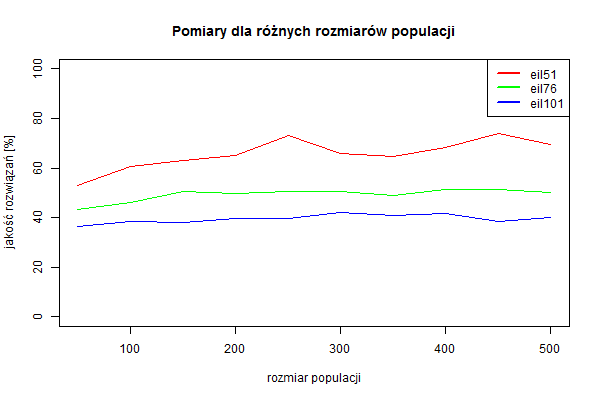
\includegraphics[width=0.95\textwidth]{./assets/tsp_pop.png}
	\caption{Jakość rozwiązań dla różnych rozmiarów populacji}
	\label{fig:tsppop}
\end{figure}

\subsection{Algorytm hybrydowy}
\paragraph{}

\begin{figure}[H]
	\centering
	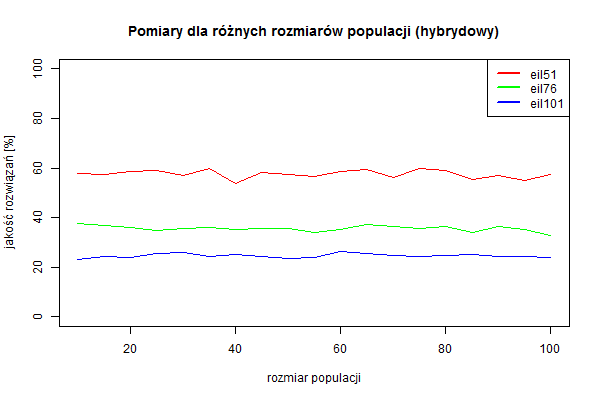
\includegraphics[width=0.95\textwidth]{./assets/tsp_pop_hyb.png}
	\caption{Jakość rozwiązań dla różnych rozmiarów populacji algorytmu hybrydowego}
	\label{fig:tsppophyb}
\end{figure}

\subsection{Optymalizacja rojem cząstek}
\paragraph{}



\newpage
\section{Podsumowanie}
\paragraph{}
W trakcie prowadzonych badań przetestowano algorytm genetyczny w~zadaniu optymalizacji dla 9 funkcji testowych. Analizie poddano wpływ zmiany każdego z~parametrów dla 4 różnych konfiguracji pozostałych wartości domyślnych.

\fbi
Wartość prawdopodobieństwa mutacji i~krzyżowania zdaje się odgrywać drugorzędną rolę. Istotne jednak by chociaż jedna z~nich była włączona z~prawdopodobieństwem większym niż 0.

\fbi
Najlepszym ustawieniem dla elityzmu jest prawdopodobieństwo rzędu 0,5.

\fbi
Z pewnością należałoby zwiększyć ilość prób poddawanych uśrednianiu gdyż dla przyjętych 20 wyniki ciągle są niestabilne. Warto by również rozważyć pomijanie kilku najlepszych i~najgorszych wyników przed uśrednianiem.

\fbi
Co ciekawe wyniki są widocznie gorsze przy konfiguracji w~której krzyżowanie jest wyłączone a~p. mutacji wynosi 0,5. Taka prawidłowość objawia się dla wszystkich badanych funkcji.

\section{Implementacja}
\paragraph{}
Poniżej (listing ~\ref{lst:skryptGlowny}) zamieszczono kod napisany w~języku R przygotowany w~celu umożliwienia przeprowadzenia pomiarów.

\lstinputlisting[label=lst:skryptGlowny,caption=Skrypt w~języku R wykorzystany do badań,firstline=1,lastline=300]{./assets/skrypt_lab35_funkcja.R}

\fbi
Skrypt przygotowano w~sposób który umożliwia w~pełni automatyczne przeprowadzenie wszystkich pomiarów. Jednocześnie wszystkie wykresy mogą być natychmiast podmienione w~sprawozdaniu. Poniżej pokrótce omówiono podstawowe parametry.


\begin{itemize}
	\item nOfRuns
	
	Ilość powtórzeń dla każdego pomiaru w~celu uśrednienia.
	
	\item colors, series
	
	Wektory kolorów i~nazw kolejnych serii pomiarowych. 
	
	\item params
	
	Macierz parametrów domyślnych algorytmu dla każdej z~serii. W każdym wierszu kolejno są zawarte: p. mutacji, p. krzyżowania, rozmiar populacji, ilość iteracji oraz kolor serii na wykresach.
	
	\item functions
	
	Wektor nazw funkcji dla których przeprowadzane są kolejno pomiary.
	
\end{itemize}

Całość informacji niezbędnych do przeprowadzenia obliczeń odczytywana jest na podstawie nazwy funkcji z~pakietu ,,globalOptTests''. Są to: rozmiar problemu (ilość parametrów), domyślne ograniczenia, wartość w~danym punkcie oraz optimum dla domyślnych ograniczeń.


\lstinputlisting[label=lst:skryptKomiwojazer,caption=Skrypt w~języku R wykorzystany do badań dla problemu komiwojażera,firstline=1,lastline=300]{./assets/skrypt_lab35_komiwojazer.R}


\newpage
\begin{thebibliography}{40}

\bibitem{test1}
Artur Suchwałko ,,Wprowadzenie do R dla programistów innych języków'' https://cran.r-project.org/doc/contrib/R-dla-programistow-innych-jezykow.pdf


\bibitem{test2}
Luca Scrucca ,,Package GA''
https://cran.r-project.org/web/packages/GA/GA.pdf

\bibitem{test3}
Surjanovic, S. \& Bingham, D. (2013). ,,Virtual Library of Simulation Experiments: Test Functions and Datasets.'' Retrieved April 3, 2017, from http://www.sfu.ca/~ssurjano.

\bibitem{test4}
Momin Jamil, Xin-She Yang ,,A literature survey of benchmark functions for global optimization problems'', Int. Journal of Mathematical Modelling and Numerical Optimisation, Vol. 4, No. 2, pp. 150–194. (2013)

\bibitem{test5}
Ajith Abraham, Aboul-Ella Hassanien, Patrick Siarry, Andries Engelbrecht, ,,Foundations of Computational Intelligence Volume 3'' (2009)

\bibitem{test6}
Onay Urfalioglu, Orhan Arikan ,,Self-adaptive randomized and rank-based differential evolution for multimodal problems'' (2011)

\end{thebibliography}

\end{document}